\documentclass{scrartcl}
\usepackage{graphicx}
\usepackage{amsmath}
\usepackage{listings}
\usepackage{mathtools}
\usepackage{physics}
\usepackage{siunitx}
\usepackage{tikz}
\usepackage{mathtools}
\usepackage{rotating}
\usepackage{hyperref}
\usepackage{fancyhdr}
\usepackage{float}

\pagestyle{fancy}
\fancyhf{}
\rhead{Jamie Grieser}
\lhead{Simulation Methods}
\rfoot{Page \thepage}

\definecolor{mygreen}{rgb}{0,0.6,0}
\definecolor{mygray}{rgb}{0.5,0.5,0.5}
\definecolor{mymauve}{rgb}{0.58,0,0.82}

\lstset{ 
	backgroundcolor=\color{white},   % choose the background color; you must add \usepackage{color} or \usepackage{xcolor}; should come as last argument
	basicstyle=\footnotesize,        % the size of the fonts that are used for the code
	breakatwhitespace=false,         % sets if automatic breaks should only happen at whitespace
	breaklines=true,                 % sets automatic line breaking
	captionpos=b,                    % sets the caption-position to bottom
	commentstyle=\color{mygreen},    % comment style
	deletekeywords={...},            % if you want to delete keywords from the given language
	escapeinside={\%*}{*)},          % if you want to add LaTeX within your code
	extendedchars=true,              % lets you use non-ASCII characters; for 8-bits encodings only, does not work with UTF-8
	frame=single,	                   % adds a frame around the code
	keepspaces=false,                 % keeps spaces in text, useful for keeping indentation of code (possibly needs columns=flexible)
	keywordstyle=\color{blue},       % keyword style
	language=Octave,                 % the language of the code
	morekeywords={*,...},            % if you want to add more keywords to the set
	numbers=left,                    % where to put the line-numbers; possible values are (none, left, right)
	numbersep=5pt,                   % how far the line-numbers are from the code
	numberstyle=\tiny\color{mygray}, % the style that is used for the line-numbers
	rulecolor=\color{black},         % if not set, the frame-color may be changed on line-breaks within not-black text (e.g. comments (green here))
	%showspaces=false,                % show spaces everywhere adding particular underscores; it overrides 'showstringspaces'
	showstringspaces=false,          % underline spaces within strings only
	showtabs=false,                  % show tabs within strings adding particular underscores
	stepnumber=2,                    % the step between two line-numbers. If it's 1, each line will be numbered
	stringstyle=\color{mymauve},     % string literal style
	tabsize=2,	                   % sets default tabsize to 2 spaces
	%title=\lstname                   % show the filename of files included with \lstinputlisting; also try caption instead of title
}

\begin{document}

\section*{Problem Sheet 9}
\subsection*{Exercise 1.1}
To do the calculations in this exercise, the routine provided on the website was used due to its better implementation and performance. 
We chose the number of cells \( N = 2000 \) for all parts of Exercise 1.1.\\
The whole source code as well as the movie are provided in the attachments.
Periodic boundary conditions have been implemented in the following way:

\begin{lstlisting}[title=Modification of the advect() function with periodic boundary conditions.,  language=Python, frame=single]
# Function to perform an advection step in Ex1.2 sheet 8
def advect(q, v, dx, dt):
	flux = np.zeros_like(v)
	ipos = np.where(v >= 0.)[0]
	ineg = np.where(v < 0.)[0]
	flux[ipos] = q[ipos]*v[ipos]
	flux[ineg] = q[ineg+1]*v[ineg]
	qnew = q.copy()
	qnew[1:-1] -= dt * (flux[1:] - flux[:-1]) / dx
	qnew[0] = qnew[-2]
	qnew[-1] = qnew[1]
	return qnew
\end{lstlisting}
The following code was used to do solve the 1D-hydrodynamics problem with a fixed step-size.
\begin{lstlisting}[title=Symmetric numerical derivative code.,  language=Python, frame=single]
def run_solver_fixed_dt():
	cs = 1  # Speed of sound is set equal to 1
	x = np.linspace(-L/2, L/2, N + 2)
	q = np.zeros((2, N + 2))
	q[0, :] = density_distribution(N, L)[:, 0]
	q[1, :] = initial_flux(N)[:, 0]
	
	snaps = [0, 10, 20, 30, 40, 50, 60, 70, 80, 90, 100]
	time = 0
	dt = 0.05
	configure_pyplot()
	for i in range(0, timesteps):
		q = hydro_iso_classic_one_timestep(q, cs, dx, dt)
		
		snap, new_dt = snapshot(time, snaps, dt)
		if snap:
			plt.plot(x, q[0, :], label='Plot of the density at ' + str(time + new_dt) + ' s')
		time += dt
	plt.legend(loc="upper right")

\end{lstlisting}
The snapshot function takes the current time and time-step as input as well as an array of the timestamps where we want to do a snapshot and then checks if the current time is close to a snapshot time and if the next step will overshoot this snapshot time. 
\begin{lstlisting}[title=Function to check whether we have to do a snapshot or not.,  language=Python, frame=single]
# Function that calculates whether we want to have to do a snapshot
def snapshot(time, snaptimes, current_dt):
	snaptimes = np.array(snaptimes)
	index = np.where((snaptimes <= (time + current_dt)) & (time <= snaptimes))[0]
	if snaptimes[index].size == 1:
		return True, np.abs(snaptimes[index] - time)[0]
	else:
		return False, 0

\end{lstlisting}
In figure \ref{fig:ex1fixed}, we can see the plots of the resulting solution fo the problem. 
We immediately see the spurious oscillations after some around \( \SI{70.0}{s} \) have passed and the waves are closing in on the boundary of the system. 
Reason for this is the limited grid resolution.
\begin{figure}[H]
	\centering
	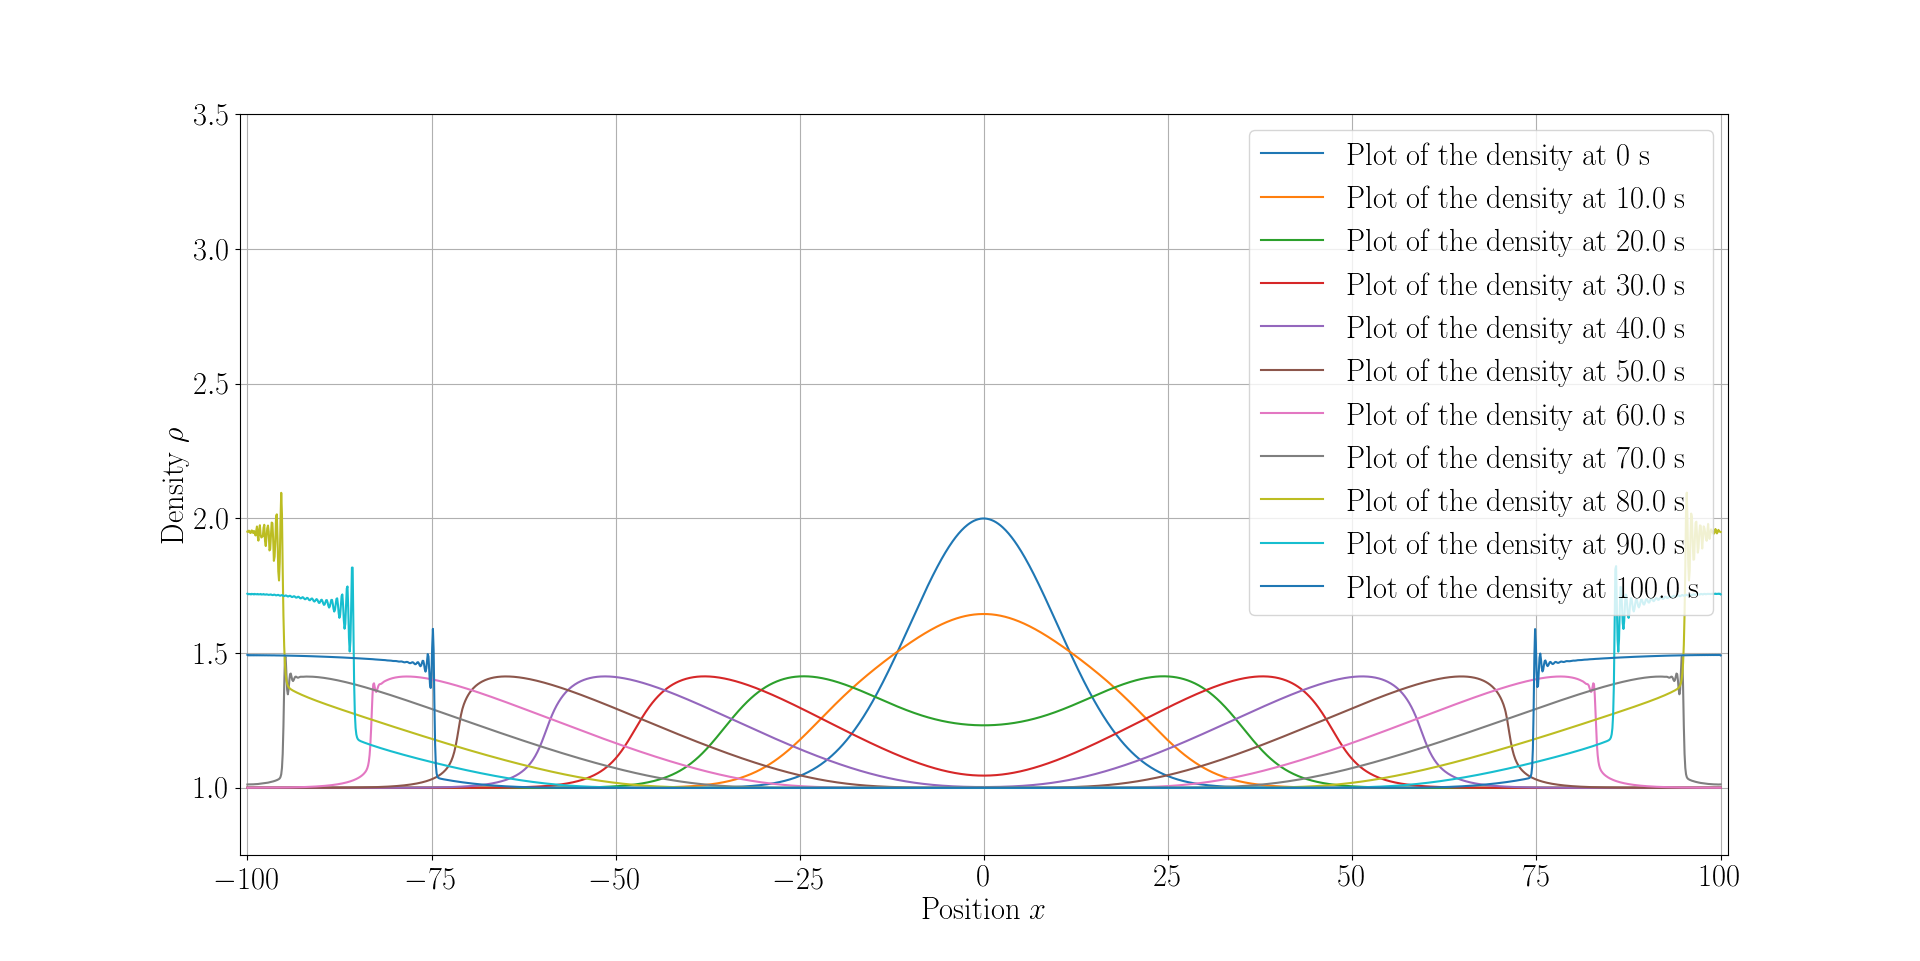
\includegraphics[width=1\linewidth]{Plots/Ex1_fixed}
	\caption{Plot of the solution for a fixed time-step size \( dt = 0.1 \). The time-step size meets the CFL-condition at all measured times and was determined experimentally.}
	\label{fig:ex1fixed}
\end{figure}

Next, we implemented a solver for the same problem with a variable time-step.
\begin{lstlisting}[title=Function that runs the simple solver with a self-adjusting time-step.,  language=Python, frame=single]
def run_solver_variable_dt():
cs = 1  # Speed of sound is set equal to 1
x = np.linspace(-L/2, L/2, N + 2)
q = np.zeros((2, N + 2))
q[0, :] = density_distribution(N, L)[:, 0]
q[1, :] = initial_flux(N)[:, 0]
snaps = [0, 10, 20, 30, 40, 50, 60, 70, 80, 90, 100]
# snaps = np.linspace(0, 250, 400)

time = 0
dt = 0.01
for i in range(0, timesteps):
	print("Time:", time, dt)
	snap, custom_dt = snapshot(time, snaps, dt)
	if snap:
		# evolve the system to the snapshot time and do a snapshot
		q = hydro_iso_classic_one_timestep(q, cs, dx, custom_dt)
		time += custom_dt
		plt.cla()
	
		configure_pyplot()
	
		plt.plot(x, q[0, :], 'b-', label='Plot of the density at ' + str(time)[0:5] + ' s')
		plt.legend(loc="upper right")
		plt.savefig('./movie/hydro_' + frame_index(i) + '.png')
		time += calculate_dt(q)
	else:
		q = hydro_iso_classic_one_timestep(q, cs, dx, dt)
		time += dt
	# Calculate next time-step
	dt = calculate_dt(q)
\end{lstlisting}
The function \textit{calculate\_dt()} was used to get the time-step size based on the CFL condition:
\begin{lstlisting}[title=Function that runs the simple solver with a self-adjusting time-step.,  language=Python, frame=single]
# Function to calculate the CFL value
def calculate_dt(q):
	if np.amax(np.abs(q[1, :])) != 0:
		cfl = dx / (np.amax(np.abs(q[1, :])))
		dt = 0.4 * cfl
	else:
		# If the velocity field is zero, start with this time-step
		dt = 0.1
	return dt
\end{lstlisting}

The result of this code is depicted in figure \ref{fig:ex1variable}.

\begin{figure}[H]
	\centering
	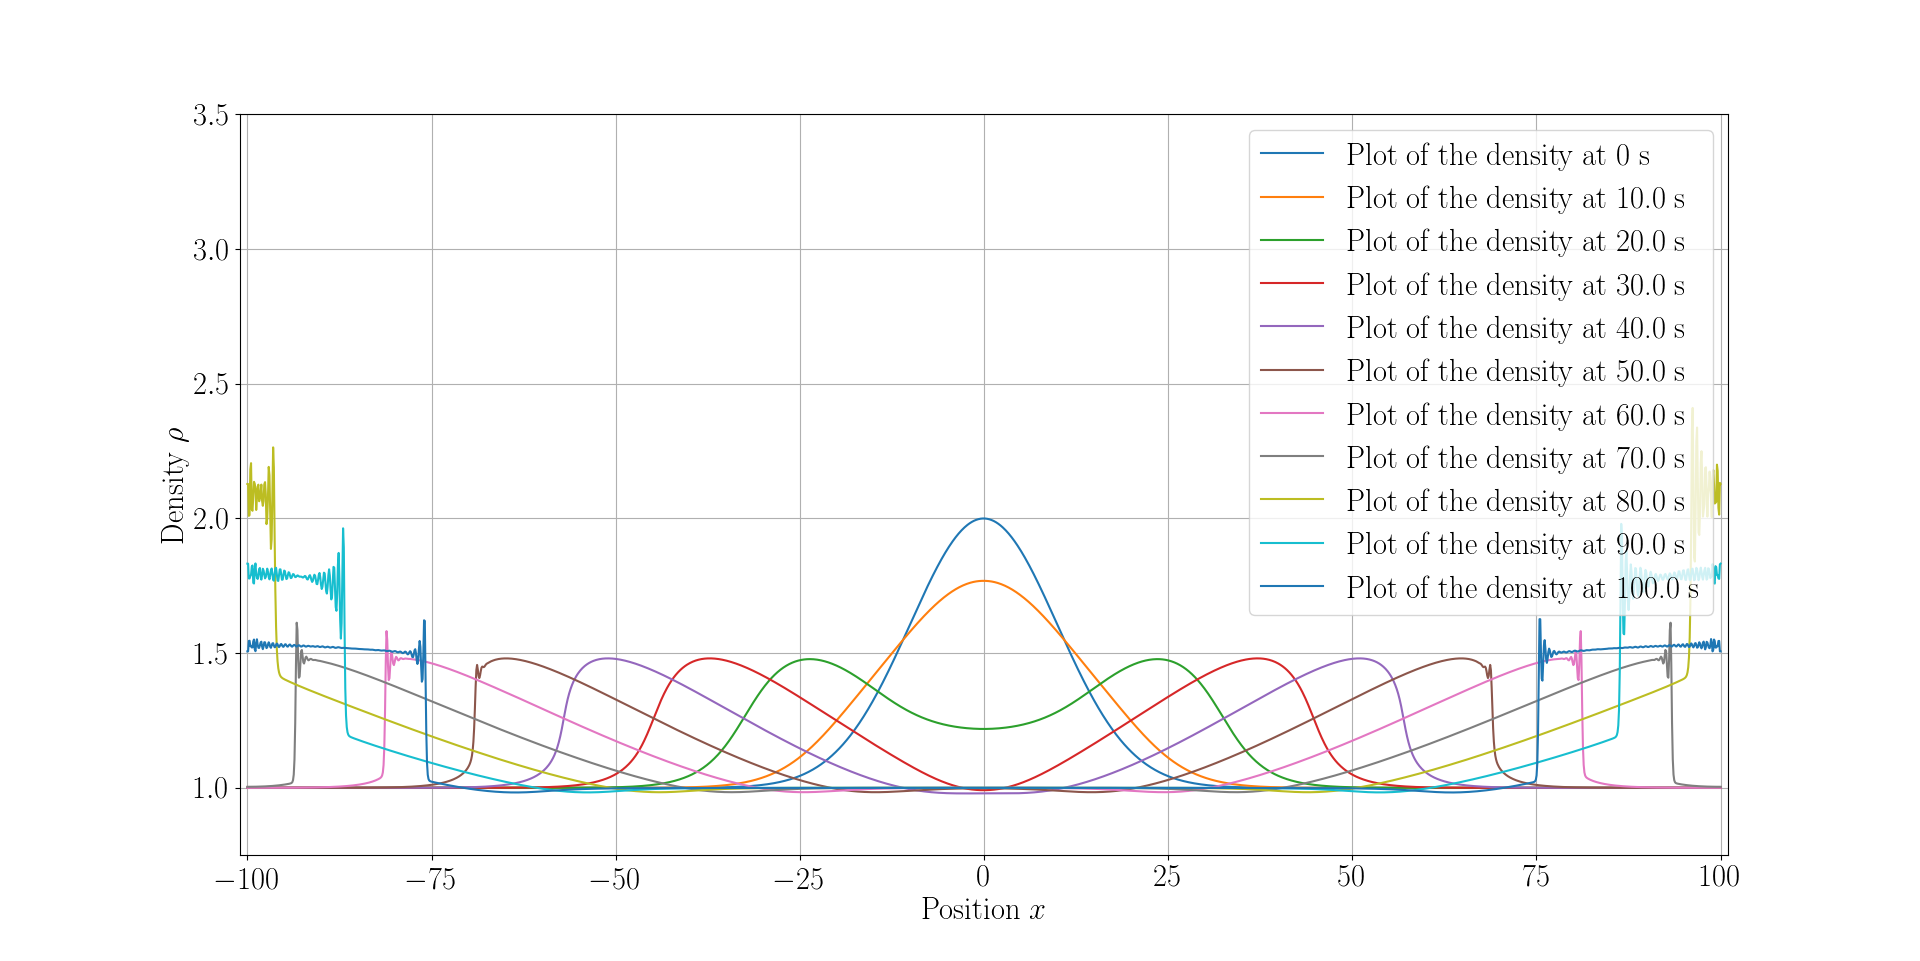
\includegraphics[width=1\linewidth]{Plots/Ex1_variable}
	\caption{Plot of the algorithm with a time-step size based on the CFL condition.}
	\label{fig:ex1variable}
\end{figure}


If we reduce the spacing of the snap-array to a smaller value we can take more pictures and make a movie of them. For example, using 

\begin{lstlisting}[language=Python, frame=single]
snaps = np.linspace(0, 150, 400)
\end{lstlisting}
we can make a movie with 400 frames evenly distributed over 150 seconds using \textit{ffmpeg}.

\end{document}
